\chapter{Resultados y discusión}\label{chapter:resultados}

Durante la implementación del proyecto, se evaluaron diversas tecnologías con el objetivo de seleccionar aquella que mejor se ajustara a los plazos de desarrollo y permitiera cumplir los objetivos establecidos. Aunque inicialmente se consideró la creación de un modelo de inteligencia artificial desde cero utilizando Python, los resultados indicaron que el tiempo necesario para entrenar el modelo y estabilizar sus respuestas era considerablemente elevado, lo que hacía inviable esta opción dentro de los plazos previstos.

Por otro lado, la implementación de modelos preentrenados, como los ofrecidos por OpenAI, resultó ser una alternativa mucho más eficiente. Estos modelos proporcionaron respuestas consistentes y claras tras un proceso de ajuste mínimo. Los resultados reflejan que, aunque fue necesario un grado de entrenamiento para adaptar los modelos a los objetivos específicos del proyecto, el tiempo total de desarrollo y ajuste fue significativamente menor en comparación con el desarrollo de un modelo desde cero. Además, la integración de estos modelos con la herramienta CASE fue fluida, lo que facilitó alcanzar los resultados esperados en un marco temporal reducido.

Para verificar el desempeño de los modelos de OpenAI integrados en la herramienta CASE, se realizó una prueba piloto con 15 estudiantes, quienes ingresaron descripciones de casos de uso relacionados con Sistemas IoT. Posteriormente, se realizó una encuesta para evaluar la satisfacción de los estudiantes y determinar si la nueva implementación de la herramienta CASE fue útil para su aprendizaje en el área de Software.

Los resultados de la encuesta, que se presentan a continuación mediante gráficos generados en R para facilitar su visualización, revelan la percepción de los estudiantes sobre la efectividad de la herramienta. Estos hallazgos permiten comprender de manera más lógica y clara los resultados obtenidos, destacando la mejora gracias a la extensión de la herramienta CASE mediante los modelos de OpenAI.

La figura \ref{fig:cap4_resultados} muestra los resultados obtenidos de la encuesta y a continuación analizaremos cada uno de ellos:

 \begin{figure}[H]  
	\centering
	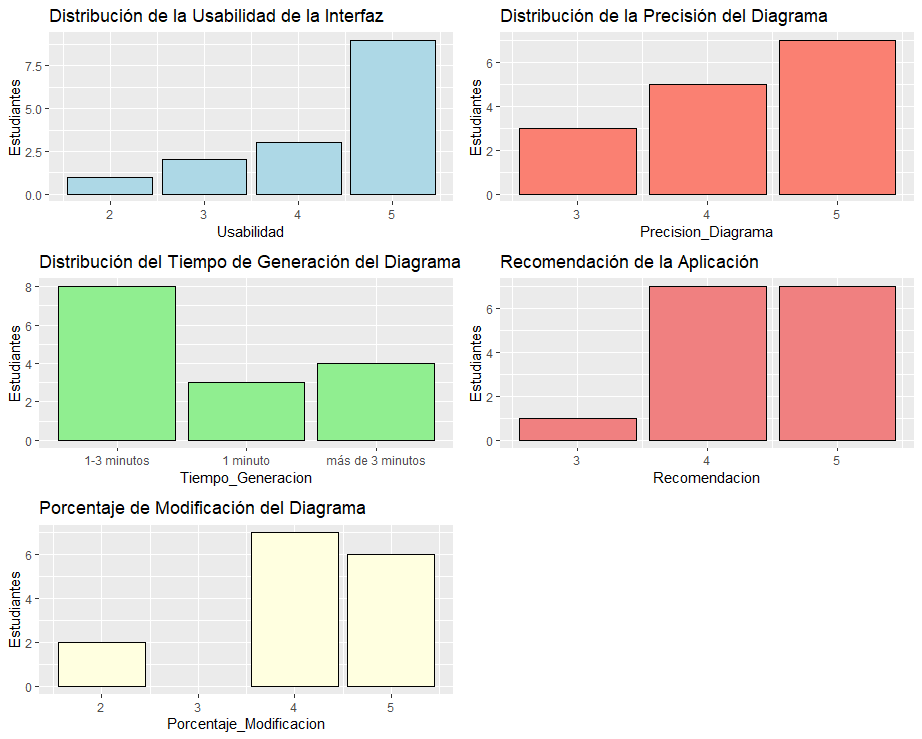
\includegraphics[width=\textwidth]{resultados.png} 
	\caption{Resultados de la encuesta.}
	\label{fig:cap4_resultados}
\end{figure}

\section{Distribución de la Usabilidad de la Interfaz}

Este gráfico muestra que la mayoría de los estudiantes (aproximadamente 8) calificaron la usabilidad de la interfaz con un 5, lo que indica una alta satisfacción con la interfaz de usuario. Un menor número de estudiantes calificó la usabilidad con 3 y 4, mientras que solo unos pocos le dieron una calificación más baja (2).

\textbf{Interpretación}: Esto sugiere que la interfaz de la herramienta es bien valorada por la mayoría de los usuarios, lo cual es un indicador positivo de la facilidad de uso del sistema implementado.

\section{Distribución de la Precisión del Diagrama}

La mayoría de los estudiantes calificaron la precisión del diagrama generado con un 5 (el puntaje más alto), seguido por un número significativo que le otorgó un 4. Solo algunos estudiantes dieron una calificación de 3 y ninguno puntuó por debajo de esto.

\textbf{Interpretación}: Los usuarios perciben que los diagramas generados por la herramienta tienen un alto nivel de precisión, lo que sugiere que el sistema cumplió bien con sus expectativas en cuanto a la representación de los casos de uso.

\section{Distribución del Tiempo de Generación del Diagrama}

La mayor parte de los estudiantes (aproximadamente 8) reportaron que el tiempo de generación del diagrama fue entre 1 y 3 minutos. Un menor número de estudiantes indicó que el tiempo fue de un minuto o de más de tres minutos.

\textbf{Interpretación}: La mayoría de los estudiantes percibió que el tiempo de generación del diagrama fue razonable y adecuado para el contexto del uso de la herramienta. Sin embargo, un pequeño grupo experimentó tiempos de generación más largos, lo que podría ser una oportunidad de mejora en la optimización de la herramienta.

\section{Recomendación de la Aplicación}

La gran mayoría de los estudiantes calificó la recomendación de la aplicación con un 4 o 5, lo que sugiere que recomendarían su uso a otros. Solo uno o dos estudiantes dieron una calificación de 3.

\textbf{Interpretación}: Esto indica una alta satisfacción general con la herramienta, lo cual es un resultado importante que refleja la utilidad percibida y la disposición de los usuarios a recomendarla.

\section{Porcentaje de Modificación del Diagrama}

Este gráfico muestra que la mayoría de los estudiantes realizaron modificaciones moderadas al diagrama, puntuando entre 4 y 5 en cuanto al porcentaje de modificación necesario. Algunos usuarios indicaron que se requirieron menos modificaciones (calificación de 3), y solo un estudiante reportó un porcentaje bajo de modificaciones.

\textbf{Interpretación}: Aunque los diagramas generados fueron precisos, aún se requirieron modificaciones para ajustarse completamente a los casos de uso. Esto indica que el sistema genera diagramas que están cercanos a la solución final, pero que necesitan pequeños ajustes por parte de los usuarios.

En general, los resultados indican que la herramienta implementada, que utiliza los modelos preentrenados de OpenAI integrados en la herramienta CASE, fue bien recibida por los estudiantes. La interfaz fue evaluada como fácil de usar, los diagramas generados tuvieron una buena aceptación, y los tiempos de generación fueron adecuados para la mayoría de los casos. Además, la mayoría de los usuarios indicaron que recomendarían la herramienta a otros. Aunque los diagramas generados necesitaban algunas modificaciones, estas eran mínimas, lo que refleja un buen desempeño en términos de exactitud.
